\documentclass[12pt]{article}    
\usepackage{ucs} 
\usepackage[utf8x]{inputenc}
\usepackage[russian]{babel}  
\usepackage{float}
\title{Псевдоэксперимент №3}
\author{Хафизов Фанис}
\usepackage[pdftex]{graphicx}
\usepackage{multirow}

\begin{document}
	\begin{figure}
		\centering
		
\includegraphics[width=0.3\linewidth]{logo}
	\end{figure}
	\maketitle
	\newpage
	\section{График представленной зависимости}
	\begin{figure}[H]
		\centering
		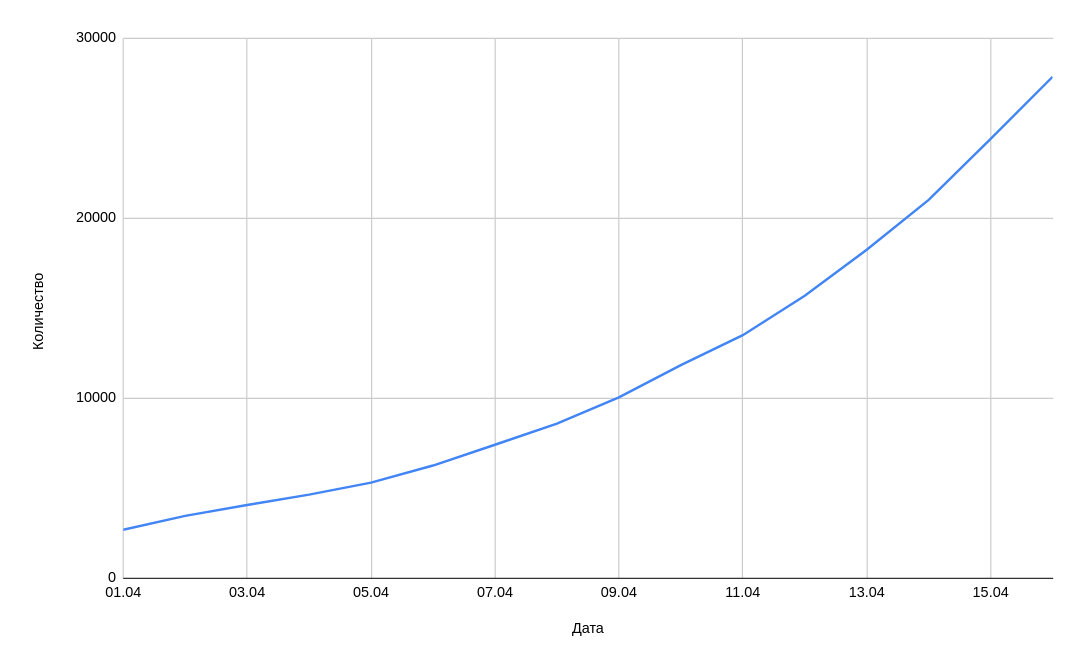
\includegraphics[width=\linewidth]{pand_graph}
		\caption{График зависимости количества заражений от дня}
	\end{figure}
	\section{Аналитическая зависимость}
	Предположим, что каждый зараженный может заразить фиксированное количество людей $k$. Тогда за каждый день количетсво зараженных будет увеличиваться в $k$ раз, и будкет зависимость вида $Q=k^{t+\phi}$, где $Q$ - количество зараженных, $t$ - время, прошедшее с начала эксперимента, $\phi$ - время, прошедшее с обнаружения первого зараженного.
	$$lg(Q) = (t+\phi)lg(k)$$
	То есть, $lg(Q)(t)$ имеет линейный вид. Построим ее график.
	\begin{figure}[H]
		\centering
		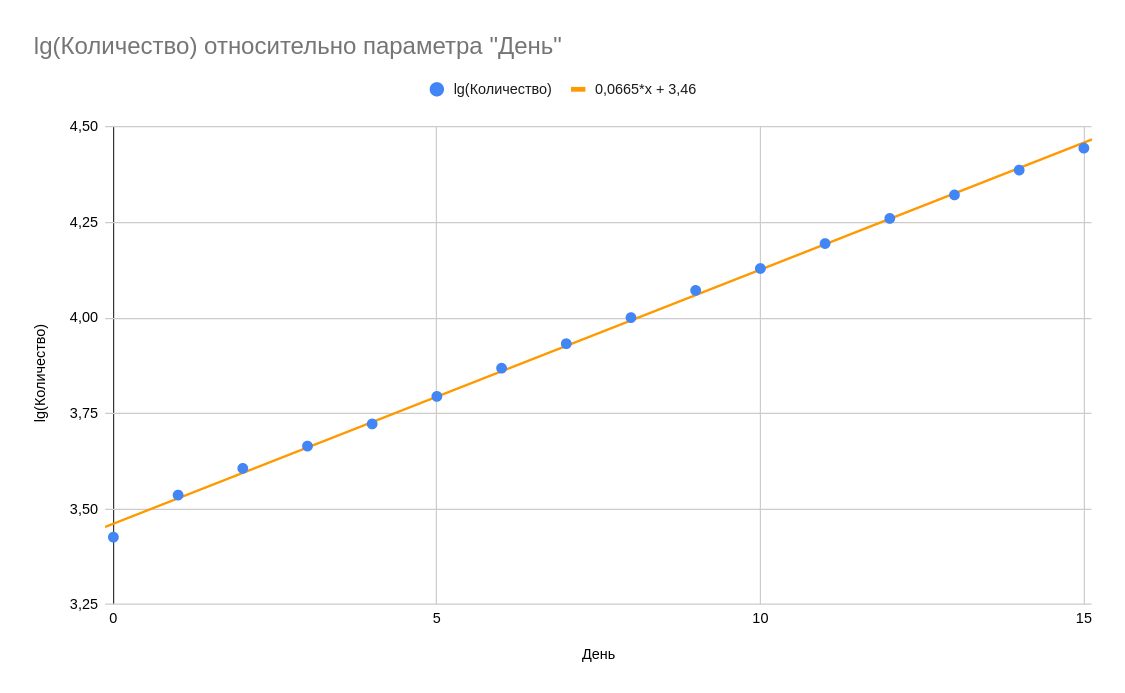
\includegraphics[width=\linewidth]{pandemia_graph}
		\caption{График зависимости десятичного логарифма количества заражений от дня}
	\end{figure}
	График показывает, что в этих осях зависимость действительно линейна.
	\section{Параметры зависимости и расчет погрешностей}
	$lg(Q) = t\cdot lg(k) + \phi\cdot lg(k)$\\
	$lg(Q) = 0,0665t + 3,45$\\
	$lg(k) = 0,0665$\\
	$k = 10^{0,0665} = 1,165$\\
	$\phi = 3,45 / 0,0665 = 51,9$(суток)\\
	$\displaystyle\Delta lg(k)=\sqrt{\frac{\sum\limits^{15}_{i=1}(\frac{lg(Q(t_{i + 1})) - lg(Q(t_i))}{t_{i+1} - t{i}} - k)^2}{15}} = 0,0126$\\
	$\Delta k = k\cdot ln(10)\Delta lg(k) = 1,165\cdot ln(10)\cdot0,0126=0,034$\\
	$k=(1,165\pm0,034)$\\
	$\varepsilon_k = \frac{\Delta k}{k} = \frac{0,034}{1,165}=3\%$\\
	$\displaystyle\Delta\phi = \frac{\sqrt{\frac{\sum\limits_{i=1}^{16}(lg(Q(t_i)) - 0,0665\cdot t_i)^2}{16}}}{lg(k)} - \phi\frac{\Delta lg(k)}{lg(k)}=9,5$\\
	$\phi=(51,9\pm9,5)$суток\\
	$\varepsilon_\phi=\frac{\Delta\phi}{\phi}=\frac{9,5}{51,9}=19\%$\\
	\section{Прогноз}
	$Q_{30} = 1,165^{29+51,9}=244625$\\
	$\Delta Q{30} = Q_{30} ln(10)\Delta lg(Q) = Q ln(10) \sqrt{\frac{\sum\limits_{i=1}^{16}(lg(Q_i)-0,0665\cdot t_i - 3,45)^2}{16}}=244625\cdot ln(10)\cdot 0,0163=9181$\\
	$Q_{30} = (244625\pm 9181)$\\
	$\varepsilon_{Q_{30}} = \frac{\Delta Q_{30}}{Q_{30}}=\frac{9181}{244625} = 4\%$
\end{document}
